%%%%%%%%%%%%%%%%%%%%%%%%%%%%%%%%%%%%%%%%%%%%%%%%%%%%%%%%%%%%%%%%%%%%%%%%%%
%
%    phase1-GO.tex  (use only for General Observer and Snapshot proposals; 
%                      use phase1-AR.tex for Archival Research and
%                      Theory proposals use phase1-DD.tex for GO/DD proposals).
%
%    HUBBLE SPACE TELESCOPE
%    PHASE I OBSERVING PROPOSAL TEMPLATE 
%     FOR CYCLE 20 (2012)
%
%    Version 1.1, February 03, 2012.
%
%    Guidelines and assistance
%    =========================
%     Cycle 20 Announcement Web Page:
%
%         http://www.stsci.edu/hst/proposing/docs/cycle20announce 
%
%    Please contact the STScI Help Desk if you need assistance with any
%    aspect of proposing for and using HST. Either send e-mail to
%    help@stsci.edu, or call 1-800-544-8125; from outside the United
%    States, call [1] 410-338-1082.
%
%
%%%%%%%%%%%%%%%%%%%%%%%%%%%%%%%%%%%%%%%%%%%%%%%%%%%%%%%%%%%%%%%%%%%%%%%%%%%

% The template begins here. Please do not modify the font size from 12 point.

\documentclass[12pt]{article}
\usepackage{phase1}
\usepackage{natbib}
\usepackage{graphicx}
\usepackage{subfigure}
\newcommand{\jnlref}[1]{\textrm{#1}}
\newcommand{\aj}{\jnlref{AJ}}
\newcommand{\araa}{\jnlref{ARA\&A}}
\newcommand{\apj}{\jnlref{ApJ}}
\newcommand{\apjl}{\jnlref{ApJ}}
\newcommand{\apjs}{\jnlref{ApJS}}
\newcommand{\ao}{\jnlref{Appl.~Opt.}}
\newcommand{\apss}{\jnlref{Ap\&SS}}
\newcommand{\aap}{\jnlref{A\&A}}
\newcommand{\aapr}{\jnlref{A\&A~Rev.}}
\newcommand{\aaps}{\jnlref{A\&AS}}
\newcommand{\azh}{\jnlref{AZh}}
\newcommand{\baas}{\jnlref{BAAS}}
\newcommand{\jrasc}{\jnlref{JRASC}}
\newcommand{\memras}{\jnlref{MmRAS}}
\newcommand{\mnras}{\jnlref{MNRAS}}
\newcommand{\pra}{\jnlref{Phys.~Rev.~A}}
\newcommand{\prb}{\jnlref{Phys.~Rev.~B}}
\newcommand{\prc}{\jnlref{Phys.~Rev.~C}}
\newcommand{\prd}{\jnlref{Phys.~Rev.~D}}
\newcommand{\pre}{\jnlref{Phys.~Rev.~E}}
\newcommand{\prl}{\jnlref{Phys.~Rev.~Lett.}}
\newcommand{\pasp}{\jnlref{PASP}}
\newcommand{\pasj}{\jnlref{PASJ}}
\newcommand{\qjras}{\jnlref{QJRAS}}
\newcommand{\skytel}{\jnlref{S\&T}}
\newcommand{\solphys}{\jnlref{Sol.~Phys.}}
\newcommand{\sovast}{\jnlref{Soviet~Ast.}}
\newcommand{\ssr}{\jnlref{Space~Sci.~Rev.}}
\newcommand{\zap}{\jnlref{ZAp}}
\newcommand{\nat}{\jnlref{Nature}}
\newcommand{\iaucirc}{\jnlref{IAU~Circ.}}
\newcommand{\aplett}{\jnlref{Astrophys.~Lett.}}
\newcommand{\apspr}{\jnlref{Astrophys.~Space~Phys.~Res.}}
\newcommand{\bain}{\jnlref{Bull.~Astron.~Inst.~Netherlands}}
\newcommand{\fcp}{\jnlref{Fund.~Cosmic~Phys.}}
\newcommand{\gca}{\jnlref{Geochim.~Cosmochim.~Acta}}
\newcommand{\grl}{\jnlref{Geophys.~Res.~Lett.}}
\newcommand{\jcp}{\jnlref{J.~Chem.~Phys.}}
\newcommand{\jgr}{\jnlref{J.~Geophys.~Res.}}
\newcommand{\jqsrt}{\jnlref{J.~Quant.~Spec.~Radiat.~Transf.}}
\newcommand{\memsai}{\jnlref{Mem.~Soc.~Astron.~Italiana}}
\newcommand{\nphysa}{\jnlref{Nucl.~Phys.~A}}
\newcommand{\physrep}{\jnlref{Phys.~Rep.}}
\newcommand{\physscr}{\jnlref{Phys.~Scr}}
\newcommand{\planss}{\jnlref{Planet.~Space~Sci.}}
\newcommand{\procspie}{\jnlref{Proc.~SPIE}}
\newcommand{\ieeesigprocm}{\jnlref{IEEE~Signal~Processing~Magazine}}
\newcommand{\cjaa}{\jnlref{Chinese J. Astron. Astrophys.}}
\newcommand{\pasa}{\jnlref{PASA}}
\let\astap=\aap
\let\apjlett=\apjl
\let\apjsupp=\apjs
\let\applopt=\ao
\newcommand{\feii}{Fe~\textsc{ii}}
\begin{document}

%   1. SCIENTIFIC JUSTIFICATION
%       (see Section 9.1 of the Call for Proposals)
%
%
\justification

Type Ia supernovae (SN Ia) are of broad interest. They are physically interesting endpoints of stellar evolution, are major contributors to galactic chemical evolution, and serve as one of astronomy's most powerful cosmological tools. 
Despite the knowledge that SN Ia are powered by runaway nuclear fusion of a massive CO white dwarf, the ignition mechanism remains a mystery. It is widely believed that either the merger of two white dwarfs or the accretion onto a white dwarf from a non-degenerate companion star leads to the required state for the white dwarf to explode; however, only the latter leaves a unique signature: a surviving companion.

While searching the remnant of SN1572 for the aforementioned surviving companion of this Type Ia supernova,  we stumbled upon a highly unusual star: Tycho-B, an A-star with a very low metallicity of [Fe/H] $\approx -1$ dex (relative to solar) {\bf[Is this right, Wolfgang??]}  and enhanced oxygen and carbon \citep{2012arXiv1210.2713K}. Such a low metallicity star should not exist anymore in the Galaxy, yet we find one within mere arc seconds of the centre of the remnant. We cannot be certain of its association with SN1572 since the distance estimates to both the star and the remnant are quite uncertain, but they are consistent within the errors.   We propose to obtain NUV spectra with STIS  to look for absorption from the ejecta and thus determine if Tycho-B is indeed located within the remnant,  or is instead a foreground or background object.

\feii\ is expected to exist in the un-decelerated ejecta of young Ia supernova remnant, and if this is the case, we can use this  to determine if Tycho-B is within the remnant.
If it is indeed within the remnant, NUV spectra (with STIS) should show blue-shifted iron absorption lines, due to cold iron along the line of sight in the  expanding supernova ejecta. No iron absorption lines would establish Tycho-B as a foreground object, while broad lines with blue and red-shifted wings would place Tycho-B in the background. For a very modest investment of two orbits, we will be able to determine if Tycho-B is within the remnant and thus a strong progenitor candidate. If Tycho-B is located in the background, absorption spectra will nevertheless be extremely valuable as a probe for the composition and kinematics of cold ejecta within the remnant---an approach that has proved extremely successful for SN 1006 \citep[e.g.][]{1988ApJ...327..164F,1993ApJ...416..247W,2005ApJ...624..189W}, but that has not been used for any other SN Ia remnant.

\vspace{-5mm}
\paragraph{What makes a Type Ia Supernova?}
SN Ia are believed to result from the explosive burning of Carbon/Oxygen white dwarfs. Theory predicts that white dwarfs will self ignite when close to the critical Chandrasekhar mass of  $1.38\,M_\odot$. 
It is believed that SN Ia originate in binary-star systems where a white dwarf accretes material from a companion star until it approaches the Chandrasekhar mass, and carbon ignites near the star's center. If the companion star is a main-sequence to red-giant star (single-degenerate scenario) we expect the companion star to survive the explosion. Another scenario sees the merger of two white dwarfs as the progenitor for SN Ia (double-degenerate scenario), which does not leave a surviving star. 
Although initially the single degenerate scenario was favoured, the last couple of years have seen a steady increase of evidence against this scenario. As of now, searches in SN1006 \citep{2012Natur.489..533G,2012ApJ...759....7K}, SN1604 (Kerzendorf. et al. 2013 in prep.) and SNR 0509-67.5 in the LMC \citep{2012Natur.481..164S} have failed to reveal a plausible surviving companion. However, \citet{2011Sci...333..856S, 2007Sci...317..924P, 2012arXiv1203.2916F} suggest that for at least a quarter of SN Ia there are signs of circumstellar interaction - suggesting a single degenerate origin. {\bf[To this  you might add Williams et al. 2011, ApJ, 741, 96, who found evidence that  RCW86 (probably = SN185 remnant) was a Type Ia inside a bubble.--FW]} In summary, both observation and theory support the two scenarios, with some community members suggesting that both channels may be responsible for the SN Ia phenomenon. This makes the identity of Tycho-B even more crucial.


\vspace{-5mm}
\paragraph{Donor Stars}
In the single-degenerate case, the consequences for the donor star post-explosion have been extensively explored by several groups. \citet{2000ApJS..128..615M} calculated the impact of a SN Ia explosion on a variety of binary companions. \citet{2001ApJ...550L..53C} have explored many of the observational consequences for a variety of possible progenitor scenarios; \citet{2004MNRAS.350.1301H} and \citet{Han:2008p726} followed the time evolution of the binary accretion in the supersoft SN Ia channel and determined the donor properties at the time of the explosion, while \citet{2003astro.ph..3660P} has explored the post-explosion evolution of the out-of-equilibrium star. \citet{2009ApJ...701.1665K} have suggested that post-explosion rotation -- a relic of tidal locking during Roche Lobe Overflow -- might be a good indicator for a donor star. 
To summarize these results, main-sequence and subgiant companions lose 10-20\% of their envelopes,  have a resulting spatial velocity of 100-300 km/s, and will have rotational velocities of 120-140 km/s; whereas a red-giant companion loses most of its hydrogen envelope, leaving a helium core (and a small amount of envelope material), with a spatial velocity of about 10-50 km/s and a rotational velocity of around 60 km/s.

\vspace{-5mm}
\paragraph{The Hunt for Donor Stars in SN1572}
Tycho's supernova (a.k.a. SN1572) is relatively close ($2.8\pm0.8$~kpc), very young, and has been confirmed as a normal Type Ia both from the remnant \citep{2006ApJ...645.1373B} and the light echo \citep{2008ApJ...681L..81R,2008Natur.456..617K}. This makes it a perfect hunting ground for donor stars.

On the basis of an unusual spatial velocity and distance compatibility with SN1572, \citet{2004Natur.431.1069R} proposed ``Tycho-G'' (by their nomenclature) to be the donor star to SN1572.  However, theory indicates that donor stars should be rapidly rotating and \citet{2009ApJ...701.1665K} found this {\bf not} to be the case for Tycho-G. Kerzendorf, et al.  (in prep.) have followed up six stars  near the center of SN1572 (including Tycho-G; see Figure 1a) with Keck HIRES  and find that five stars rotate with surface velocity less than 6.5\,km/s and show no other strong peculiarities . But there is one star in this sample that stands out: Tycho-B.

\vspace{-5mm}
\paragraph{The curious case of Tycho-B}
Tycho-B is a rapidly rotating, $v_{{\rm rot}}\, {\rm sin}(i)=170$~km/s, A-Star ($T_{\rm eff}=10,700$\,K) with  log($g$) = 4.1, making it a very promising candidate. In particular,  it is located within arc seconds of the X-ray centre of the remnant, and at $d = 1.8\pm 0.8$~kpc its distance is compatible (just) with the remnant of SN1572 ($d = 2.8\pm0.8$~kpc). The possibility that Tycho-B is at the same distance as the remnant is greater than what these numbers suggest: Tycho-B's distance was calculated assuming a mass (2.4\,$M_\odot$) taken from standard stellar evolution (BASTI isochrones), which probably do not fully apply here. Finally, Tycho-B shows an extremely unusual abundance pattern of low metallicity ([Fe/H]$\; =-1$) and relatively high C and O abundances.

Despite these remarkable features, the standard single-degenerate scenario seems to fail \citep{2012arXiv1210.2713K} for Tycho-B.  In this scenario, the rotational velocity is tidally induced, and hence  results in a coupling of spatial velocity and rotational velocity.  Thus if the rapidly rotating Tycho-B is the surviving companion, we would  expect it to have a high spatial velocity---which it lacks.  {\bf[You need a reference for this.  Have limits been set on proper motion?  Presumably your spectra show radial velocity is small. -- FW}

However, a ``normal" A-Star model for Tycho-B seems to fail as well, mostly due to the extreme low metallicity. This conundrum has already triggered theoretical speculations \citep[e.g.][]{2012arXiv1212.2662T}. To lend support or rule out any scenarios it is crucial to find out if SN1572 could have been responsible for the current state of Tycho-B.

In summary, finding such a rare type of star close to the remnant of a supernova is tantalizing evidence (the probability of a chance alignment are very slim) for an involvement with SN1572, but requires the proof that Tycho-B is within the remnant.

\vspace{-5mm}
\paragraph{In or out?}
Establishing Tycho-B's location to be within the remnant would provide very convincing evidence for interaction of SN1572 and Tycho-B. 
\cite{1988ApJ...327..164F,1993ApJ...416..247W, 2005ApJ...624..189W} all have used UV absorption line studies, in particular the \feii\ lines at 2383 and 2600~\AA) to probe the structure of the SN1006 remnant along several lines of sight. Two background objects near the projected centre of SN1006  (the Schweizer-Middleditch 1980 star and a $z \approx 1$ QSO) show absorption lines with very broad red and blue components (from the advancing and receding side of the ejecta; see Figure 1b).  We would expect similar features in the NUV spectrum of Tycho-B if it is more distant than SN1572.   If it is located  within the remnant it should  show only blue-shifted absorption features, while if it is a foreground object it will show no such broad absorption features at all. A similar technique to establish a distance has been tried by \citet{2007PASJ...59..811I} for  several stars in SN1572 (not including Tycho-B).  No strong absorption features were seen, but their spectra reached only relatively weak Fe~\textsc{i} lines at 3720 and 3860 \AA, with relatively poor signal-to-noise near the atmospheric cut-off.  
 Far stronger absorption can occur  from permitted transitions that connect to the ground state, such as the 2383 and 2600~\AA\ lines in \feii.  
SN1572 is an ideal candidate for such observations, it is young enough that the reverse shock has not penetrated back to the explosion \citep[current radius 183\arcsec;][]{2005ApJ...634..376W}, which would  ionize much of the \feii. We propose to take two orbits of low-resolution STIS observations of Tycho-B to look for these absorption features. If found,  this proves an involvement of Tycho-B with SN1572 and may provide the missing piece that links some SN Ia with the single degenerate scenario.

{\bf[Another ref. to add:  Schweizer, F. \& Middleditch, J. 1980, ApJ, 241, 1039.]}

\begin{figure}[h!] %  figure placement: here, top, bottom, or page
\vspace{-0mm}
\subfigure[Overview of inner region of the remnant of SN1572. Tycho-B, the most promising candidate for a donor star, is located very close to the X-ray geometric center (arrow indicates Tycho-B).]{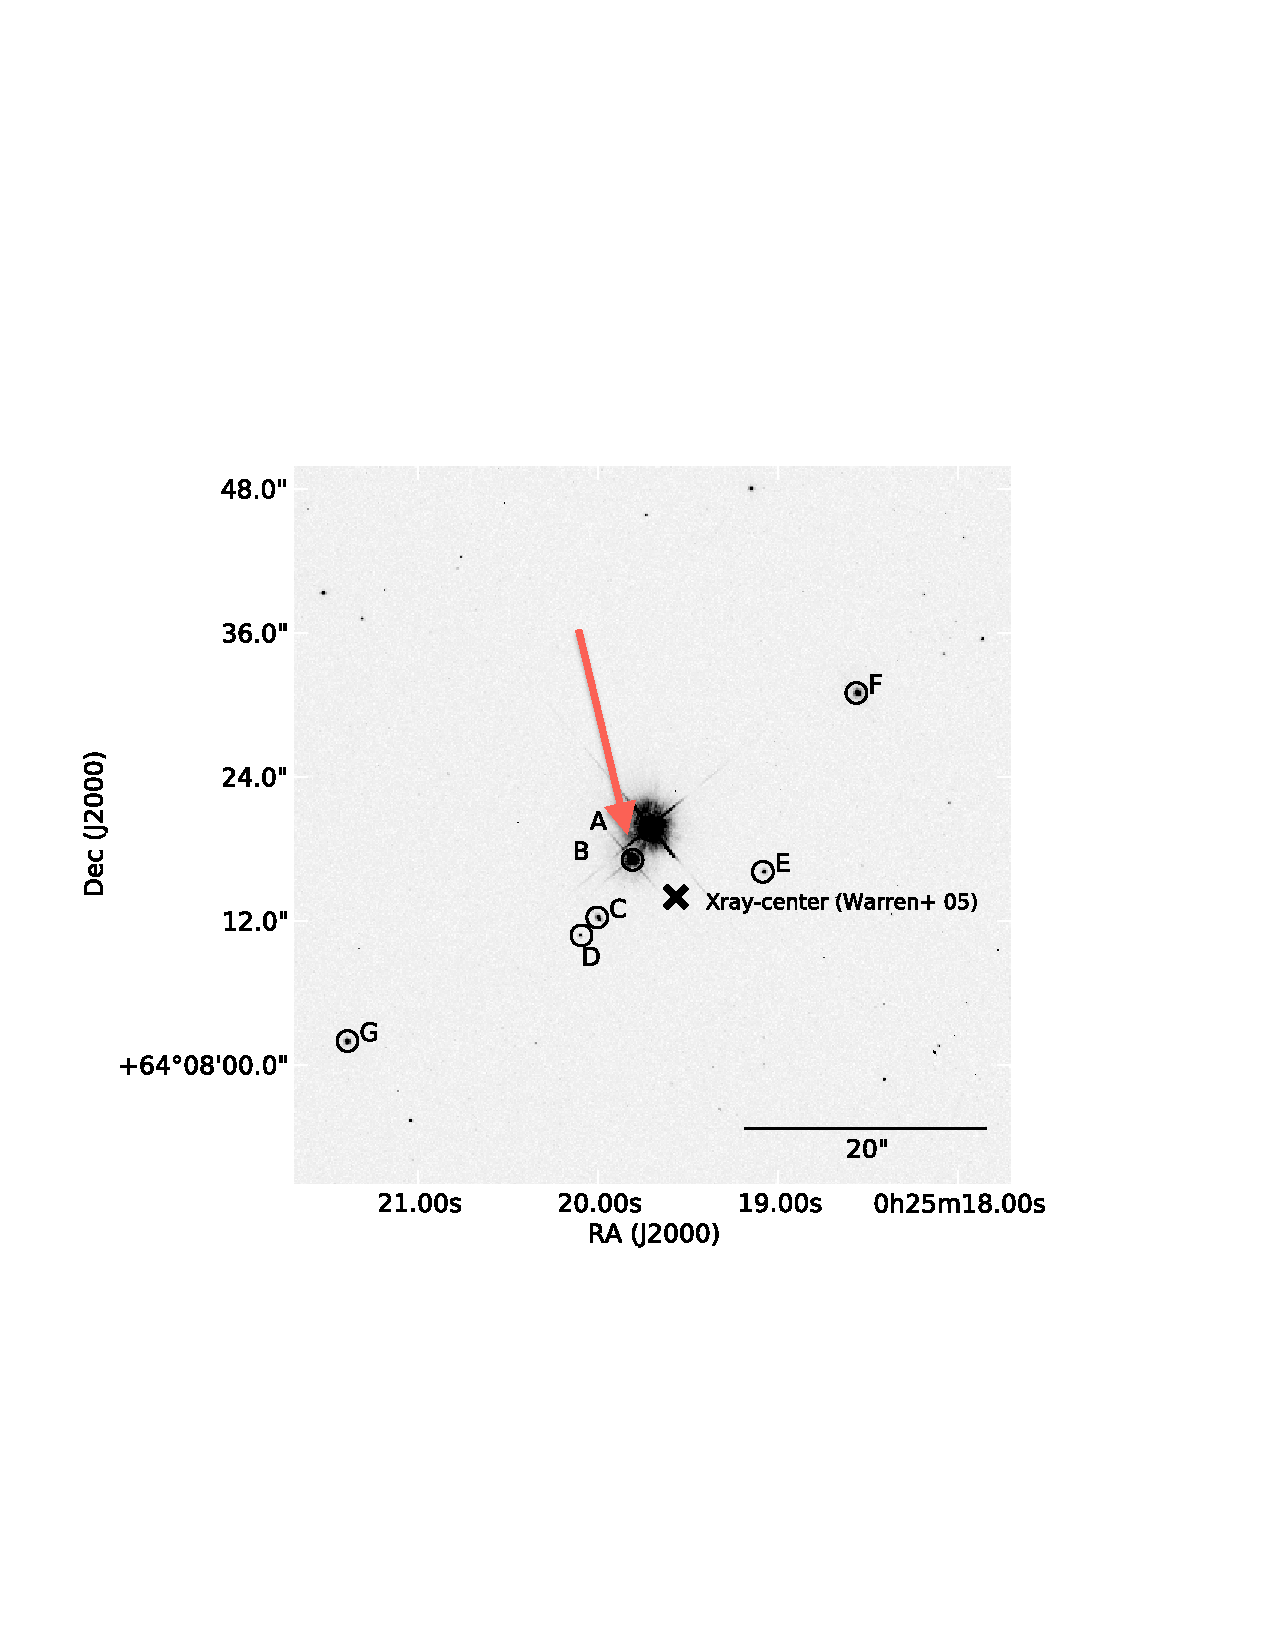
\includegraphics[width=0.4\textwidth]{Plots/overview_sn1572.pdf}}
\subfigure[\feii\ absorption features of the remnant on a background UV source \citep{1993ApJ...416..247W}]{
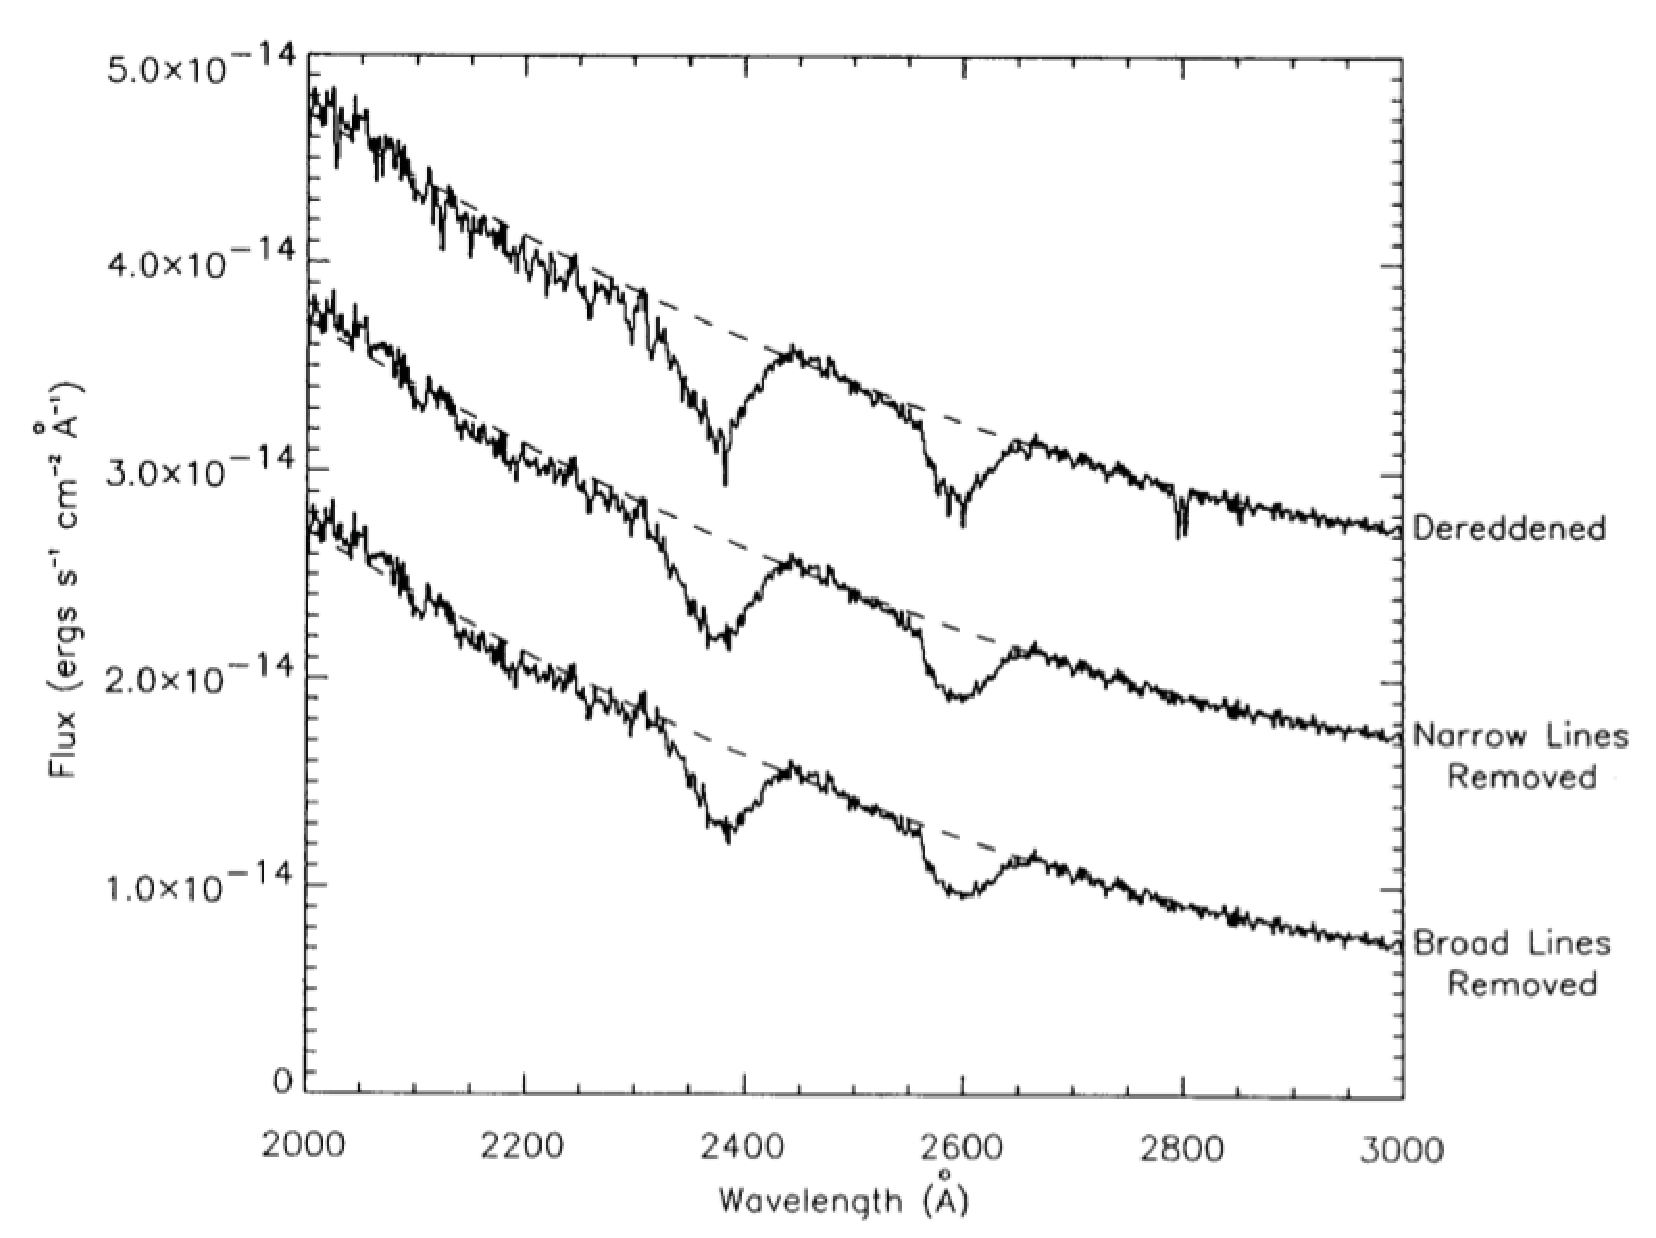
\includegraphics[width=0.45\textwidth]{Plots/Wu_1997_fig_2.pdf}}
\vspace{-.2cm}
\end{figure}

\newpage
         % Do not delete this command.
% Enter your scientific justification here. 

%%%%%%%%%%%%%%%%%%%%%%%%%%%%%%%%%%%%%%%%%%%%%%%%%%%%%%%%%%%%%%%%%%%%%%%%%%%

%   2. DESCRIPTION OF THE OBSERVATIONS
%       (see Section 9.2 of the Call for Proposals)
%
%
\describeobservations   % Do not delete this command.
% Enter your observing description here.

We propose an observation that is not possible from the ground, due to the atmospheric cut-off in the UV. The position of Tycho-B allows it to be observable for 51 minutes per orbit (shortened from 59 minutes due to ``Increased scheduling flexibility'' -- a requirement for our RA). We propose two orbits of observations.

To establish Tycho-B's position in the remnant we need a UV spectrum that covers the \feii\ absorption features at 2600\,\AA\ with a S/N of roughly 10. The absorption features are broadened by several 1000~km/s (see Figure 1b) and so we opt for the low-resolution grating G230L (R=700 or 400 km/s) on MAMA (enhanced sensitivity in this wavelength region compared to CCD), with a slit geometry of 52\arcsec\ x 0.5\arcsec\ (relatively isolated star). Using the STIS ETC (ver 21.1) and assuming V = 15.4 \citep{2004Natur.431.1069R}, with Pickles Models A0V, and E(B-V) of 0.85 (reddening estimated by fitting a flux-calibrated spectrum of Tycho-B; consistent with Tycho-E - a background source) we need  4,210.8~s (http://etc.stsci.edu/etc/results/STIS.sp.486061/). 
In addition, we have done photometry on F336W (U-Band) WFPC2 images (HST Prop ID 6435) and find a U=16.78. We have used this value in the ETC with the same settings as above and for a required S/N=10 we obtain 4,006.7~s (http://etc.stsci.edu/etc/results/STIS.sp.486086/). In our further calculations we will continue using the U magnitude.


Our target with `increased scheduling flexibility' (a requirement for our target RA) is visible for 51 minutes per orbit. Using two orbits with an overhead of 20 minutes (6 minutes guide star acquisition), we can obtain 2x1860~s of integration time. This results in a S/N of  9.6, appropriate for our requirements. We will orient the STIS slit to minimize the light that enters the spectrograph from the very bright star Tycho-A (U=15.96).   {\bf[Add a note here about the separation between Tycho-A and Tycho-B.  Are they far enough apart that the 0.5\arcsec slit is OK? -- FW]}


%%%%%%%%%%%%%%%%%%%%%%%%%%%%%%%%%%%%%%%%%%%%%%%%%%%%%%%%%%%%%%%%%%%%%%%%%%%

%   3. SPECIAL REQUIREMENTS
%       (see Section 9.3 of the Call for Proposals)
%
%
\specialreq             % Do not delete this command.
% Justify your special requirements here, if any.

%%%%%%%%%%%%%%%%%%%%%%%%%%%%%%%%%%%%%%%%%%%%%%%%%%%%%%%%%%%%%%%%%%%%%%%%%%%

%   4. COORDINATED OBSERVATIONS
%       (see Section 9.4 of the Call for Proposals)
%
%
\coordinatedobs          % Do not delete this command.
% Enter your coordinated observing plans here, if any.

%%%%%%%%%%%%%%%%%%%%%%%%%%%%%%%%%%%%%%%%%%%%%%%%%%%%%%%%%%%%%%%%%%%%%%%%%%%

%   5. JUSTIFY DUPLICATIONS
%       (see Section 9.5 of the Call for Proposals)
%
%
\duplications           % Do not delete this command.
% Enter your duplication justifications here, if any.

%%%%%%%%%%%%%%%%%%%%%%%%%%%%%%%%%%%%%%%%%%%%%%%%%%%%%%%%%%%%%%%%%%%%%%%%%%%


%   6. PAST HST USAGE
%       (see Section 9.8 of the Call for Proposals)
%
%        List here the program numbers and data status for all accepted GO/AR/SNAP 
%        programs of the PI in at least the last four HST Cycles. Include a list of refereed publications 
%        resulting from these programs.       
%
%       Note that the description of past HST usage  DOES NOT count against the page limits of the proposal.
%
\pasthstusage  % Do not delete this command.
The PI has not used HST in the past, however Winkler and Long both have experience with STIS spectroscopy.
% Enter your Past HST Usage and current commitments for the PI
% and other key investigators.

%%%%%%%%%%%%%%%%%%%%%%%%%%%%%%%%%%%%%%%%%%%%%%%%%%%%%%%%%%%%%%%%%%%%%%%%%%%
\newpage
\bibliographystyle{hapj}
\bibliography{hst_phasei_tychob}
\end{document}          % End of proposal. Do not delete this line.
                        % Everything after this command is ignored.

